\documentclass[12pt]{../notes}

% Command for Questions
%\question{}

% Command for Notes
% \note{}

% Code to create a minipage where you can type in class notes. 
%%\begin{minipage}[l][2cm][c]{\textwidth}
%\begin{comment}

%\end{comment}
%%\end{minipage}

\usepackage{listings}

% In order for the minted code to run, we had to create a new compilation routine called pdflatex+shellEscape.
% This includes a --shell-escape command which should ONLY be used when pygmentized is required as it compromises security. 
% We also had to add pygmentize (a python package) to the system path (BEFORE miktex) and then restart the computer. 
\usepackage{minted}
\usemintedstyle{borland}
\lstset{language=SAS, 
  breaklines=true,  
  basicstyle=\ttfamily\bfseries,
  columns=fixed,
  keepspaces=true,
  identifierstyle=\color{blue}\ttfamily,
  keywordstyle=\color{cyan}\ttfamily,
  stringstyle=\color{purple}\ttfamily,
  commentstyle=\color{green}\ttfamily,
  } 
  
% \begin{minted}{sas}
% \end{minted}


% Begin Document
%==============================================================================
\begin{document}
% Include the Title of the Handout
\ntitle{4.1: Penalized Regression}

% Include Numbered Sections
\section{Why Penalized Regression?}


\nspace 
\question{What are some undesirable consequences of having estimates of $\beta_k$'s with inflated variance?}

 \begin{minipage}[l][5cm][c]{\textwidth}
%\begin{comment}
\note{
\bi
\item Interpretation: the sign/magnitude of the estimated coefficients could be misleading or non-intuitive
\item Stability: Coefficients could change drastically for small changes in the training data, which makes it hard to persuade others that the model form is correct. 
\item Variable selection: When the number of candidate explanatory variables is large, inflated variance may cause us to throw the ``best'' predictor variables out in a stepwise search. 
\ei
}
%\end{comment}
\end{minipage}

\nspace 

\question{Why is it critical that we \textbf{standardize} our variables prior to using any of the penalized regression techniques?}

 \begin{minipage}[l][2cm][c]{\textwidth}
%\begin{comment}
\note{The penalty terms do not respect differences in the \textbf{scale} of variables. Variables with a small range of values will be unfairly punished if we do not standardize.}
%\end{comment}
\end{minipage}


\nspace
  
\question{Which of the following is NOT a good scenario to used penalized regression techniques? Why?
\begin{enumerate}
\item Facebook is trying to create a model to predict the likelihood of a user responding positively to a certain type of ad. 
\item The Huntsman Cancer institute is trying to determine which active genes in a person’s DNA increase the likelihood of Pancreatic cancer. 
\item The USU Agriculture Experiment Station is trying to determine if a change in the composition of feed significantly influences the milk output of dairy cows.
\end{enumerate}
}

\begin{minipage}[l][4cm][c]{\textwidth}
%\begin{comment}
\note{
\textbf{3} is the correct answer because:
\bi 
\item This scenario is an experiment rather than an observational study. 
\item We are interested in the significance of an effect, rather than accurate predictions. 
\ei
}
%\end{comment}
\end{minipage}

\newpage
\question{Which method does NOT get estimated coefficients exactly equal to zero as the penalty parameter increases? Why?
\begin{itemize}
\item Ridge Regression
\item LASSO 
\item Elastic Net
\end{itemize}}

\begin{minipage}[l][3cm][c]{\textwidth}
%\begin{comment}
\note{Ridge Regression: The use of the squared penalty term makes it nearly impossible for coefficients to converge to be exactly equal to zero as the penalty parameter increases.}
%\end{comment}
\end{minipage}

\question{Given the following output, determine the value of the intercept for the following ridge regression model.}

\begin{figure}[H]
\centering
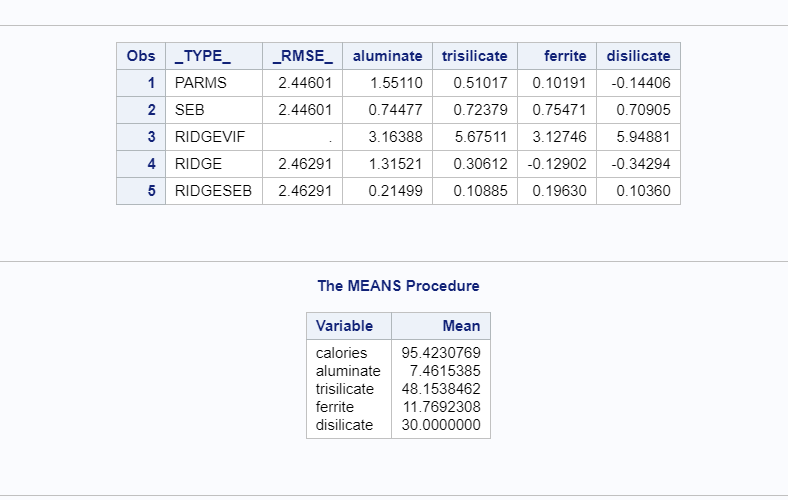
\includegraphics[width=\textwidth]{../figures/module4/ridge_regression_intercept.png}
\end{figure}

\begin{minipage}[l][3cm][c]{\textwidth}
%\begin{comment}
\note{$$95.423 - 1.315*7.462 - 0.306*48.154 + 0.129*11.769 + 0.343*30 = 82.684$$}
%\end{comment}
\end{minipage}




% End the Document
%==============================================================================
\end{document}